\chapter{Computational Modeling}
\section{Deterministic Models}
We start by considering a deterministic model, which is a system of ordinary
differential equations (ODEs) that describe the time evolution of the
concentrations of the species in the system.

The main issue of deterministic models is \textbf{time}, which is represented
as a discrete variable.

The standard tool use to model deterministic models is the \textbf{ordinary
    differential equations} (ODEs). The ODEs are a set of equations that describe
the time evolution of the concentrations of the species in the system.

A different approach is to use \textbf{discrete event simulation} (DES), which
are a queue of events generated by a sources and processed by components. In this
representation, time is usually a derived notion, for example observing the
sequence of events.

\subsection{Stem Cell Differentiation}
The first model we consider is the stem cell differentiation model. The
\textbf{stem cell} differentiate into \textbf{progenitor cells}, which in turn
differentiate into \textbf{regular cells}.

The division or proliferation of stem cell can be:
\begin{itemize}
    \item \textbf{Symmetric}: the stem cell divides into two stem cells.
    \item \textbf{Asymmetric}: the stem cell divides into one stem cell and one regular cell.
    \item \textbf{Envirormentally Asymmetric}: the stem cell divides into one
          stem cell and one progenitor cell.
\end{itemize}

A first simple model of stem cell can be represented by a finite state machine
describe in Figure \ref{fig:stem_cell_fsm}.

\begin{figure}[!ht]
    \centering
    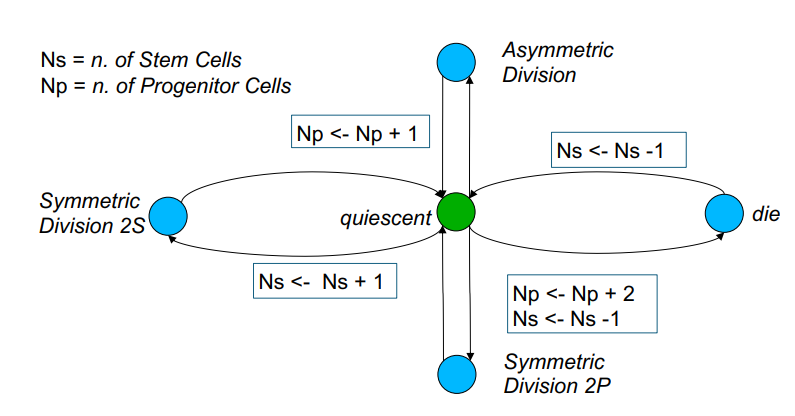
\includegraphics[width=.7\textwidth]{img/stemcellsFSA.png}
    \caption{Stem Cell Finite State Machine}
    \label{fig:stem_cell_fsm}
\end{figure}

In this example we don't consider the time. Time can be model considering an
exponential delay to the transition. Moreover, we can associate a different
probability to each transition, so we have a transition system (Markov Chain).
\subsection{Implementing a simulator}
In order to implement a simulator we need to define what means for us to run a
simulation. We can define a simulation as a sequence of events that can be
described by numerically solving a set of ODEs or by tracking the sequence of
events in a DES. This produce a \textbf{trace} of the simulation.

A trace is a sequence of vectors of values, where each vector represents the
state of the system at a given time. The trace can be used to analyze the
behavior of the system.

The engine of a simulator is essentially a loop where is body determines the
type of simulator we are using.
\subsubsection{Finite State Automata Simulator}
To implement a finite state automata simulator we need to define the following
elements:
\begin{itemize}
    \item \textbf{Specification}: first we need to define a set of finite
          automata, each represented by a matrix.
    \item \textbf{Engine}: check the set of all the enabled transitions from the
          current state and produce the next state.
    \item \textbf{Specification}: sources, computing units and sinks.
    \item \textbf{Trace}: a sequence of states.
\end{itemize}
\subsection{Deterministic Simulations}
In a deterministic simulation we want to solve a set of ODEs for what is known
as an initial value problem is the following:
\begin{equation}
    \begin{cases}
        \frac{dy(t)}{dt} = f(y(t), t) \\
        y(0) = c
    \end{cases}
\end{equation}
where $c$ is a constant and $t$ represent the time.

Based on the previous definition of simulators, we can define a deterministic
simulator as a simulator that produces a trace of the system by solving a set of
ODEs. This is composed by the following elements:
\begin{itemize}
    \item \textbf{Specification}: the ODEs and the initial conditions.
    \item \textbf{Engine}: which evaluate at discrete time steps the value of
          the function and of its derivative. For doing this we can use the Euler
          or the Runge-Kutta method.
\end{itemize}
\subsubsection{Euler Method}
The Euler method is a simple method to solve ODEs. It is based on the following
formula:
\begin{equation}
    y_{t + 1} = y_n + h \cdot f(y_n, x_n)
\end{equation}
the indices denote the $i-th$ computation and $h$ is the integration step. This
method is not recommended because it accumulate errors.
\subsubsection{Runge-Kutta Method}
The Runge-Kutta method is a more sophisticated method to solve ODEs. It is based
on the following formula:
\begin{equation}
    y_{n + 1} = y_n + \frac{1}{6} \left( k_1 + 2k_2 + 2k_3 + k_4 \right) + O(h^5)
\end{equation}
where:
\begin{itemize}
    \item $k_1 = h \cdot f(y_n, x_n)$
    \item $k_2 = h \cdot f(y_n + \frac{k_1}{2}, x_n + \frac{h}{2})$
    \item $k_3 = h \cdot f(y_n + \frac{k_2}{2}, x_n + \frac{h}{2})$
    \item $k_4 = h \cdot f(y_n + k_3, x_n + h)$
    \item $O(h^5)$ is the error term.
    \item $h$ is the integration step.
\end{itemize}
\subsection{Hybrid Systems}
Hybrid systems are systems that combine continuous and discrete dynamics. In
particular, they mix finite state automata with continuous systems.

We can define an Hybrid System as a computational tool that switches among
different sets of ODEs based on the state of the system. An advantage of this is
that can express exponential delays.

We can model the stem cell population model as an hybrid system where we have
only one differential continuous variable which is time. With this we can add to
the model an exponential decay rate.

There are several numerical problems with hybrid systems, for example the
\textbf{guard crossing} problem, which is when the system crosses a guard
condition. This can be solved by using a \textbf{zero-crossing algorithm}.
\section{Stochastic Models}
In the deterministic models, fixing the initial conditions fixes the dynamics of
the system. In the stochastic models, for the same initial conditions,
quantitatively different outcomes are possible due to random occurrences of
events.

An example of stochastic model is the \textbf{Markov Chain}, which is a
stochastic process that satisfies the Markov property. Each Markov Chain is
describe by a transition matrix $P$ where $P_{ij}$ is the probability of
transition from state $i$ to state $j$.

Let's call the \textbf{state vector} $v$, this vector essentially represent a
probability distribution over the states of the system. Using this information
we can be obtained by multiplying the state vector by the transition matrix,
in order to obtain the next state vector. This process can be represented using
the following formula:
\begin{equation}
    v_{n} = v_0 \cdot P^n
\end{equation}
If $v\times P = v$ then $v$ is called a \textbf{steady state} distribution vector.
\begin{note}
    It can also be seen that $v$ is an eigenvector of $P$. The steady state does
    not imply a flat behavior, it can be a distribution.
\end{note}
\subsection{Petri Nets}
An example of stochastic model can be represented by the \textbf{Petri Nets}.
Some particular type of Petri Nets allow us to add information to the Markov
Chain, for example:
\begin{itemize}
    \item \textbf{Timed Petri}: which can enable simultaneous transitions. The
          one with the shortest deadline will be served first.
    \item \textbf{Stochastic Petri Nets}: the delay associated with a transition
          $T$ is a random variable $X_T$.Its probability density function is
          assumed to be an exponential distribution with parameter $\lambda$.

          In this case we have the problem of choose which transition to serve
          first in the case that multiple transitions are enabled. To solve this
          we can assume that there will be no conflict situation, so stochastic
          Petri Nets are equivalent to Markov Chains.
\end{itemize}

Stochastic Petri Nets enable quantitative analysis method where only the stochastic
rate constant need to be known.
\subsection{Stochastic Simulation}
Since many biological processes involve a small number of molecules, in order to
represent them we need to use a stochastic model.

There are many ways to construct stochastic models and many of them are based on
the \textbf{Gillespie algorithm}. This algorithms are very useful to take in
account the effects the effects of very small numbers of molecules with respect
to very high concentrations of other compounds.

The goal is to describe the evolution of a system $X(t)$ from some give initial
state $X(0) = x_0$ where $x_0$ is the number of molecules of each species in the
system.

In the system we have a set of reactions $R_i$ that can occur with a rate $c_i$.
Each reaction is characterized by two mathematical entities:
\begin{enumerate}
    \item The \textbf{state change vector}
          \begin{equation*}
              \beta_i = \left( \beta_{1i}, \beta_{2i}, \ldots, \beta_{Ni} \right)
          \end{equation*}
          where $\beta_{ji}$ is the change in the number of molecules of species
          $j$ due to the occurrence of reaction $i$.

          All the $\beta_i$ are collected in a matrix $\beta$ that is called the
          \textbf{stoichiometry matrix}.
    \item The \textbf{propensity function} $a_j(x)dt$ which is the probability
          that, given $X(t) = x$, one occurrence of reaction $j$ ($R_j$) will
          happen somewhere inside a volume $V$ in the next infinitesimal time
          interval $[t, t + dt)$.
\end{enumerate}

Since we do not know the precise position and velocity of each molecules in $V$,
we can only predict the probability of a reaction to occur in the next time
interval. We can only hope to compute the probability:
\begin{equation}
    P(x, t| x_0, t_0)
\end{equation}

To formulate the description of constitutes progress in a time slice $dt$ we need
to take in account the following:
\begin{itemize}
    \item We can have that no reaction occurs in the time slice $dt$ which can
          be described by the following formula:
          \begin{equation}
              P(x, t | x_0, t_0) \cdot \left(1 - \sum_{i=1}^M a_i(x)dt\right)
          \end{equation}
    \item Another case is that a reaction $R_i$ occurs in the time slice $dt$.
          This can be described by the following formula:
          \begin{equation}
              P(x - \beta_i, t + dt | x_0, t_0) \cdot a_i(x) (x - \beta_i)dt
          \end{equation}
          since we have $M$ reactions, so we must sum all the terms above.
\end{itemize}
If we put all together we obtain the \textbf{Chemical Master Equation}:
\begin{equation}
    P(x, t + dt|x_0, t_0) = P(x, t | x_0, t_0) \cdot \left(1 - \sum_{i=1}^M a_i(x)dt\right)
    + \sum_{i=1}^M (P(x - \beta_i, t | x_0, t_0) \cdot a_i(x) (x - \beta_i)dt)
\end{equation}
which can be rewritten as:
\begin{equation}
    \frac{dP(x, t + dt|x_0, t_0)}{dt} = \sum_{i=1}^M \left[ a_i(x - \beta_i)P(x -
        \beta_i, t|x_0, t_0) - a_i(x)P(x, t|x_0, t_0) \right]
\end{equation}
This equation is analytically unsolvable, so we need to use a numerical method
to solve it. The most common method is the \textbf{Gillespie algorithm}.